\documentclass[11pt]{ctexart}
\usepackage[margin=1in]{geometry}
\usepackage{amsmath,amssymb,booktabs,graphicx,float,xurl}
\usepackage[hypertexnames=false]{hyperref}
\setlength{\emergencystretch}{6em}
\title{Luca 缺陷技术速度分区图（跨报告、固定 full-FPT 公平口径）}
\author{valley-k-small 自动化基准}
\date{\today}
\begin{document}
\sloppy
\maketitle
\section{研究范围与公平口径}
主胜负指标仅比较完整 FPT 竞争者：sparse exact recursion 与 Luca defect-reduced 路线。
线性方程法仅作为 MFPT 参考，不参与完整 FPT 胜负判定。
统一使用固定时窗口径与比例指标 $R=\text{sparse}/\text{luca}$，跨 family 结论不混合绝对秒数。
\section{方法与计时协议}
计时采用 warm-up 1 次 + 实测 3 次取中位数。
Luca 模式规则：defect pairs $\le 120$ 用 full；否则用 sampled-$z$ 外推估计。
估计式：$t_{\mathrm{est}}=t_{\mathrm{setup}}+(t_{\mathrm{eval}}/n_z)\,m+t_{\mathrm{fft}}$。
\section{主结果}
汇总中位数 $R=0.0005$（均值 0.0198），Luca 胜率 $P(R>1)=0.000$。
全局判定：No Luca winning region under fixed-T full-FPT fairness.
估计校验：n=8，中位相对误差=0.126（25\% 阈值判定：通过）。
\section{图件}
\begin{figure}[H]\centering
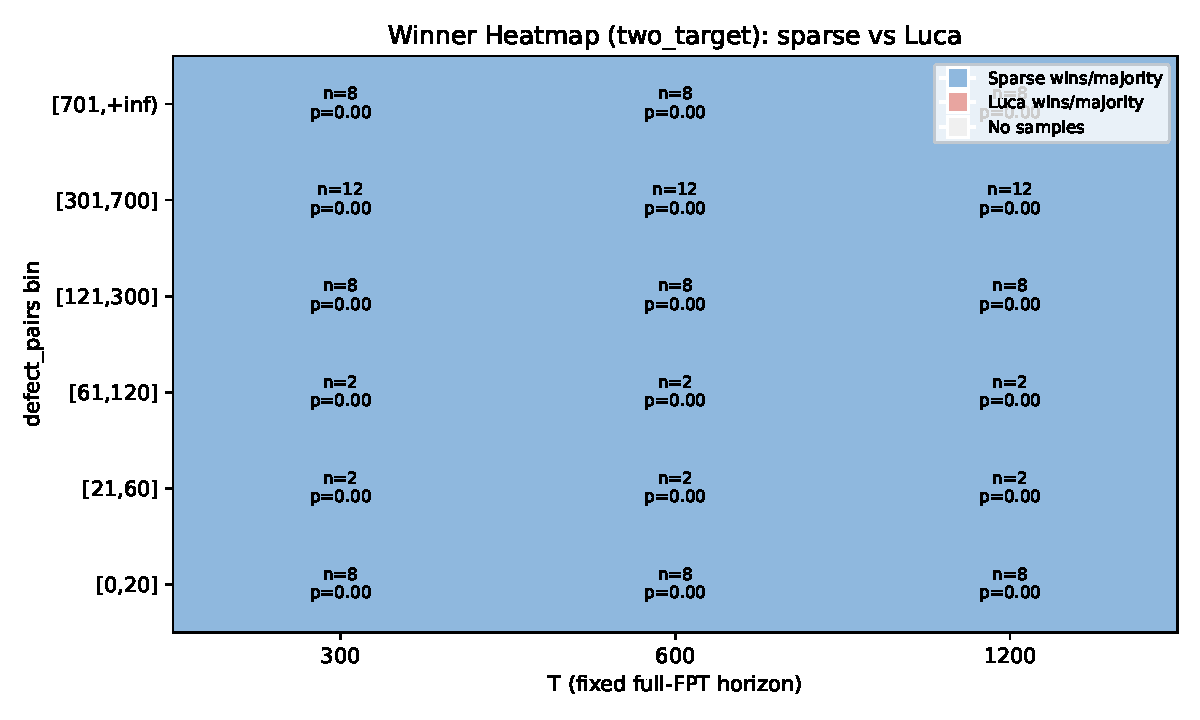
\includegraphics[width=0.9\linewidth]{figures/regime_winner_heatmap_two_target.pdf}
\caption{two-target 样本上的 winner heatmap。}
\end{figure}
\begin{figure}[H]\centering
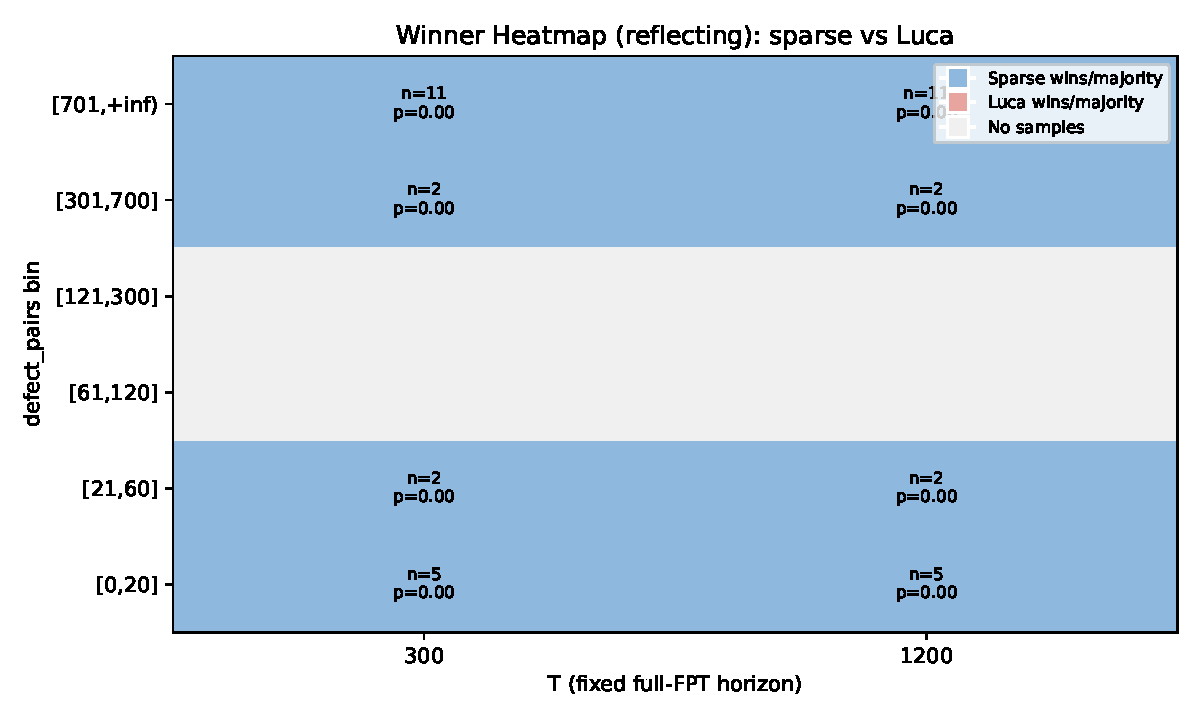
\includegraphics[width=0.9\linewidth]{figures/regime_winner_heatmap_reflecting.pdf}
\caption{reflecting 样本上的 winner heatmap。}
\end{figure}
\begin{figure}[H]\centering
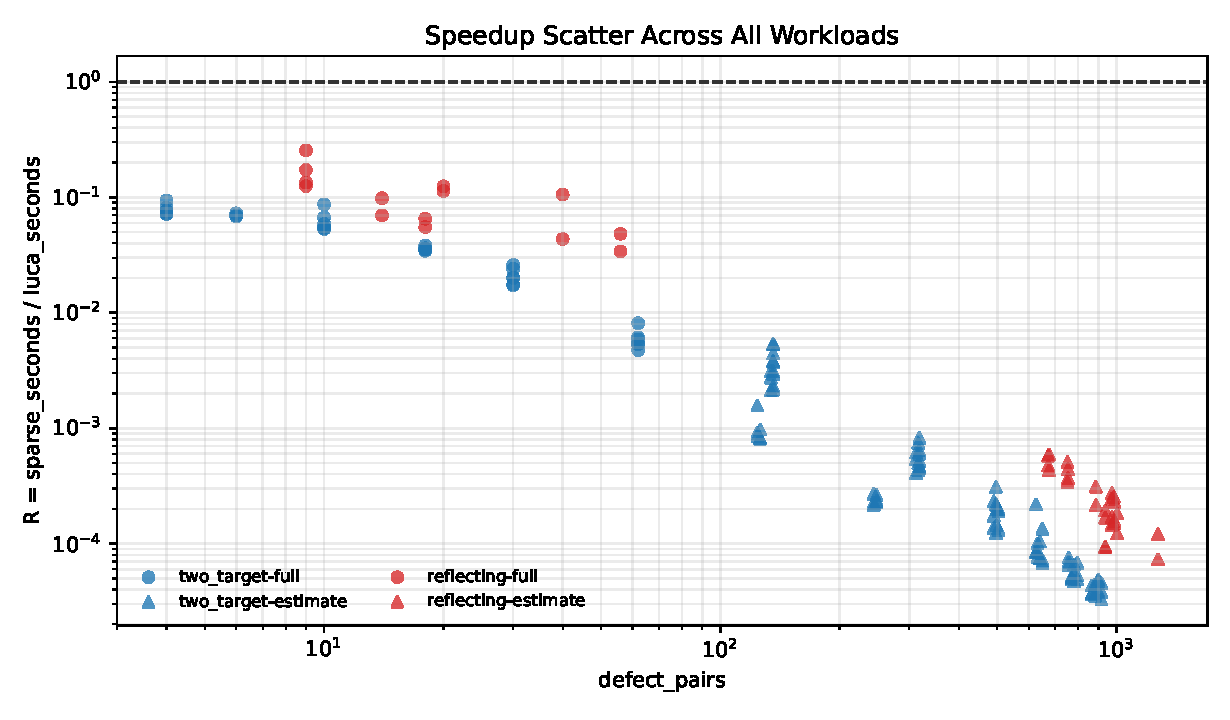
\includegraphics[width=0.9\linewidth]{figures/regime_speedup_scatter_all.pdf}
\caption{全样本速度比散点图（区分 full/estimate 模式）。}
\end{figure}
\begin{figure}[H]\centering
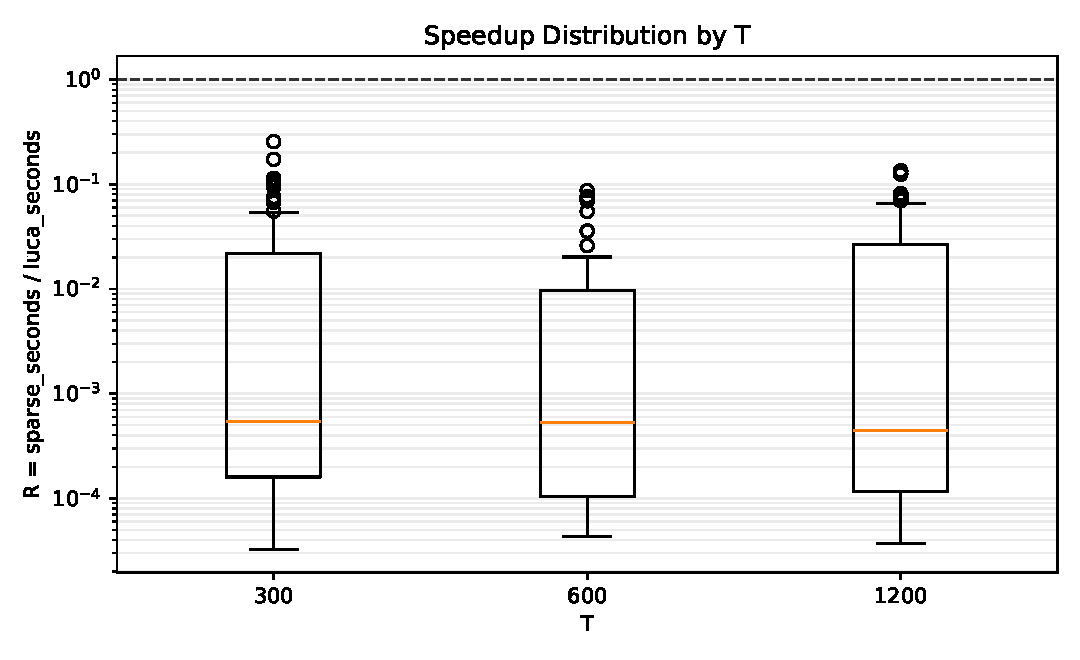
\includegraphics[width=0.8\linewidth]{figures/regime_speedup_box_by_T.pdf}
\caption{按固定时窗 $T$ 的 $R$ 分布。}
\end{figure}
\begin{figure}[H]\centering
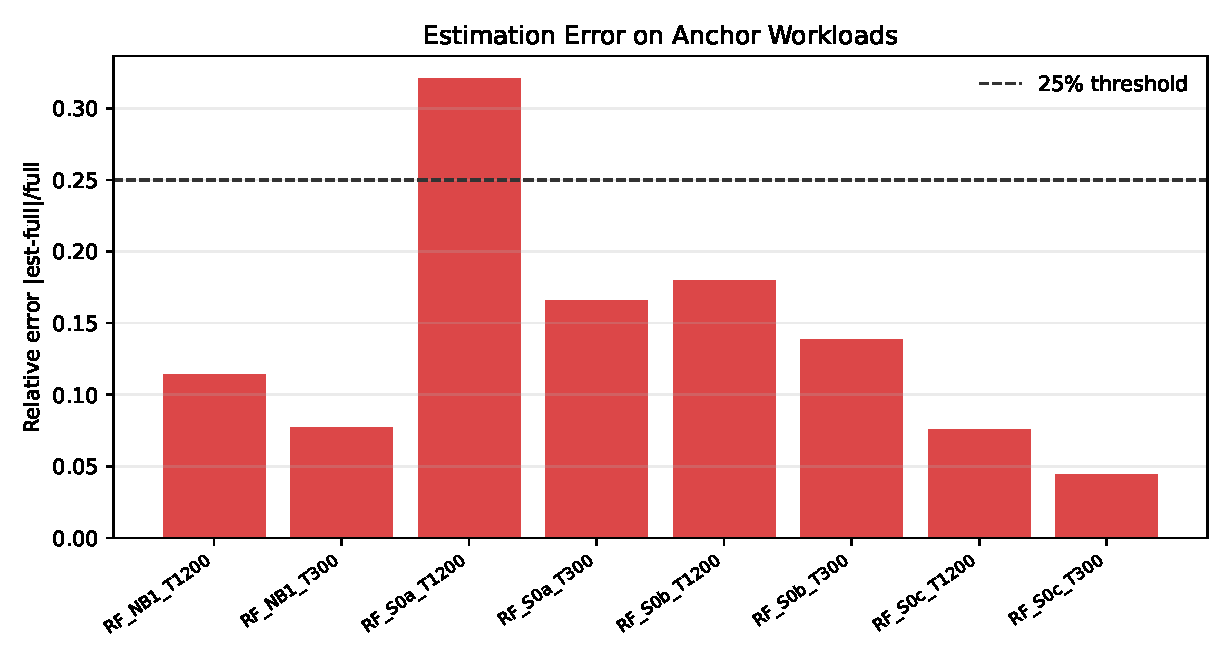
\includegraphics[width=0.8\linewidth]{figures/regime_estimation_error_anchor.pdf}
\caption{锚点 workload 上 full 与 estimate 的相对误差。}
\end{figure}
\begin{figure}[H]\centering
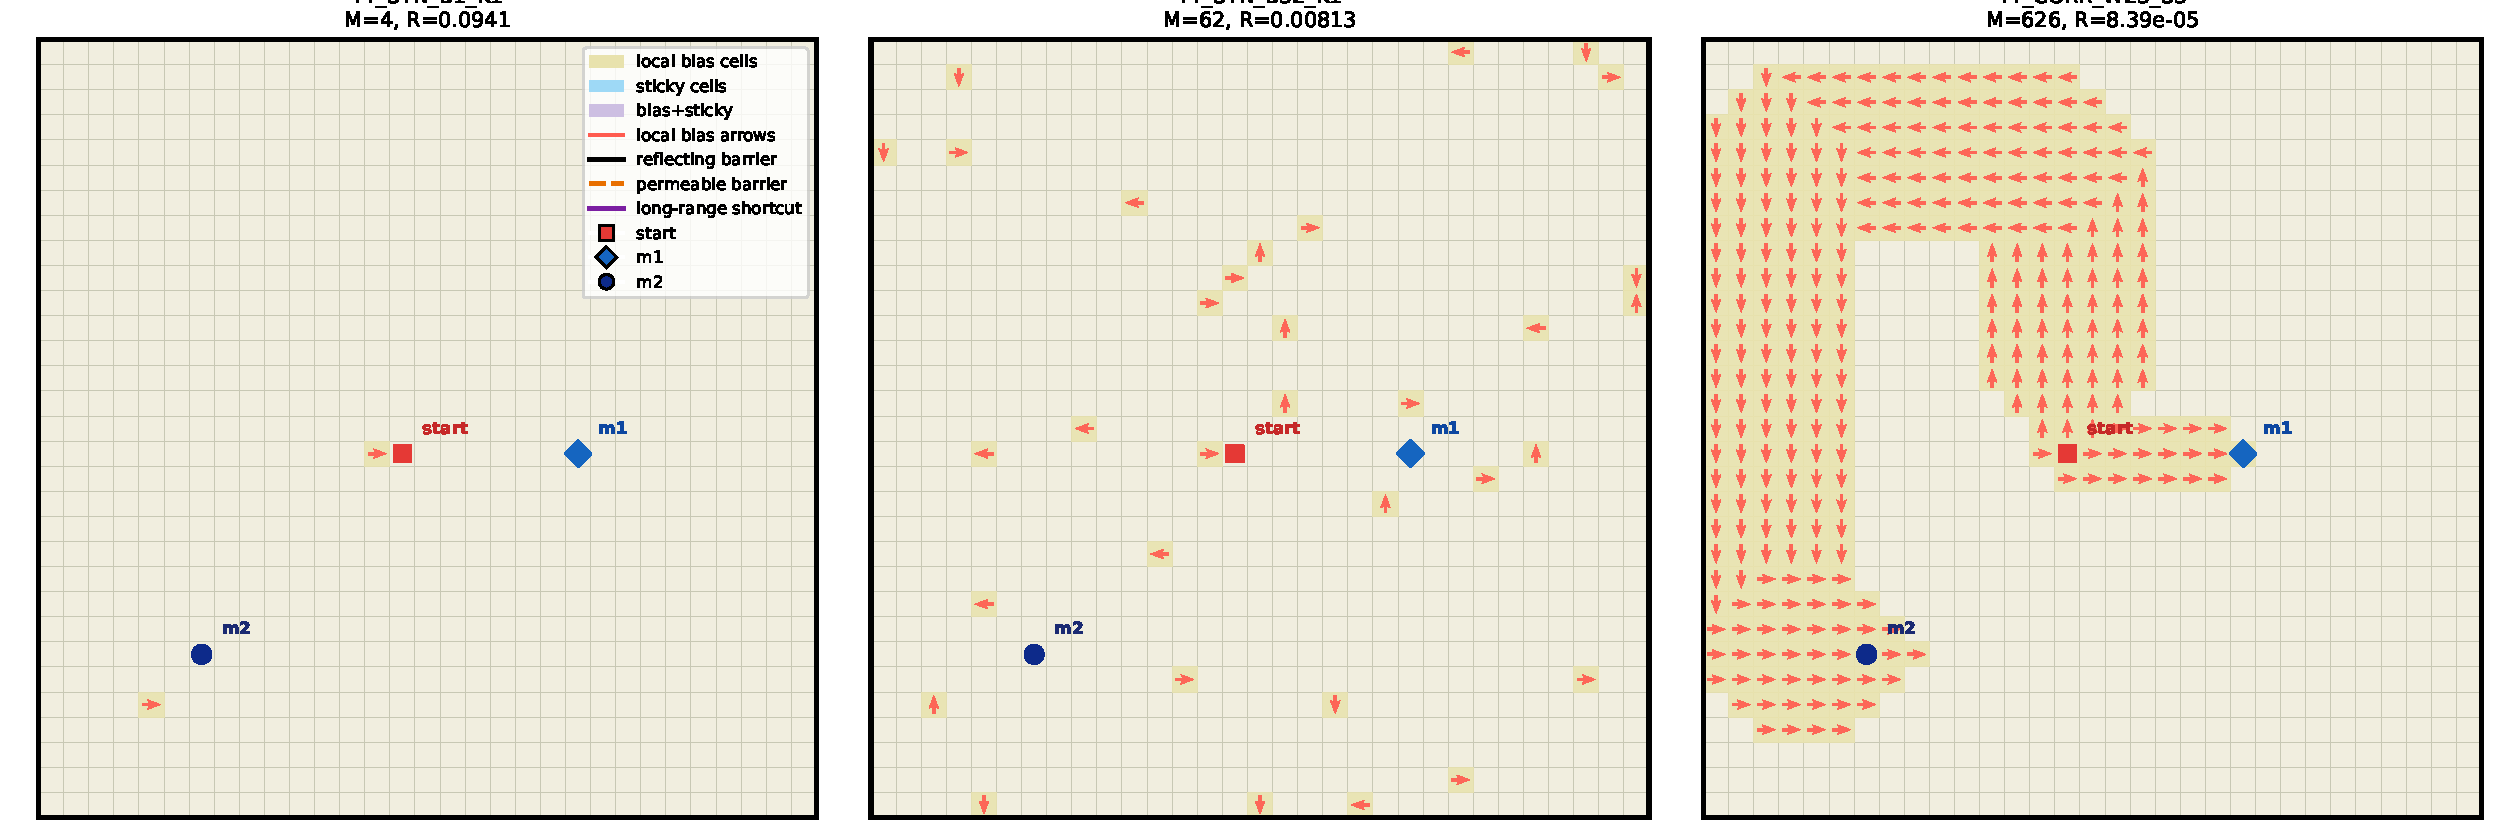
\includegraphics[width=0.98\linewidth]{figures/regime_config_examples.pdf}
\caption{低/中/高缺陷代表性配置图（复用现有风格工具）。}
\end{figure}
\section{表格}
\begin{table}[H]
\centering
\small
\caption{按缺陷分箱与时窗分组的运行比摘要。}
\resizebox{\linewidth}{!}{\begin{tabular}{lccccc}
\toprule
Defect bin & T & n & Median $R$ & Mean $R$ & $P(R>1)$ \\
\midrule
\texttt{[0,20]} & 300 & 13 & 0.0734 & 0.0919 & 0.000 \\
\texttt{[0,20]} & 600 & 8 & 0.0705 & 0.0628 & 0.000 \\
\texttt{[0,20]} & 1200 & 13 & 0.0727 & 0.0779 & 0.000 \\
\texttt{[121,300]} & 300 & 8 & 0.0019 & 0.0021 & 0.000 \\
\texttt{[121,300]} & 600 & 8 & 0.0015 & 0.0019 & 0.000 \\
\texttt{[121,300]} & 1200 & 8 & 0.0020 & 0.0021 & 0.000 \\
\texttt{[21,60]} & 300 & 4 & 0.0329 & 0.0472 & 0.000 \\
\texttt{[21,60]} & 600 & 2 & 0.0231 & 0.0231 & 0.000 \\
\texttt{[21,60]} & 1200 & 4 & 0.0290 & 0.0304 & 0.000 \\
\texttt{[301,700]} & 300 & 14 & 0.0002 & 0.0003 & 0.000 \\
\texttt{[301,700]} & 600 & 12 & 0.0002 & 0.0003 & 0.000 \\
\texttt{[301,700]} & 1200 & 14 & 0.0003 & 0.0003 & 0.000 \\
\texttt{[61,120]} & 300 & 2 & 0.0068 & 0.0068 & 0.000 \\
\texttt{[61,120]} & 600 & 2 & 0.0057 & 0.0057 & 0.000 \\
\texttt{[61,120]} & 1200 & 2 & 0.0053 & 0.0053 & 0.000 \\
\texttt{[701,+inf)} & 300 & 19 & 0.0002 & 0.0002 & 0.000 \\
\texttt{[701,+inf)} & 600 & 8 & 0.0000 & 0.0001 & 0.000 \\
\texttt{[701,+inf)} & 1200 & 19 & 0.0001 & 0.0001 & 0.000 \\
\bottomrule
\end{tabular}
}
\end{table}
\begin{table}[H]
\centering
\small
\caption{锚点配置运行时基线。}
\resizebox{\linewidth}{!}{\begin{tabular}{lcccccc}
\toprule
Anchor & Defects & Sparse(s) & Dense(s) & Full AW(s) & Luca(s) & Linear(s) \\
\midrule
low\_defect (TT\_SYN\_B1\_K1\_T300) & 4 & 0.0029 & 0.0050 & 22.9998 & 0.0416 & 0.0147 \\
high\_defect (TT\_CORR\_W23\_S2\_T300) & 632 & 0.0034 & 0.0065 & 22.2596 & 36.4872 & 0.0168 \\
\bottomrule
\end{tabular}
}
\end{table}
\section{实务建议矩阵}
\begin{table}[H]
\centering
\small
\begin{tabular}{@{}lp{0.64\linewidth}@{}}
\toprule
任务类型 & 推荐方法 \\
\midrule
固定有限时窗下的完整 FPT 曲线 & 默认采用 sparse exact recursion；仅在缺陷极稀疏且锚点校验通过时考虑 Luca。 \\
只关心 MFPT/splitting & 线性方程法（不参与 full-FPT 胜负判定）。 \\
需要变换域并且缺陷稀疏 & 可用 Luca defect-reduced AW，但需保留 estimate/full 校验。 \\
高缺陷走廊类配置 & 优先 sparse recursion；计入 setup/eval 后 Luca 常不占优。 \\
\bottomrule
\end{tabular}
\end{table}
\section{复现信息}
核心数据文件：\path{data/manifest.csv}、\path{data/runtime_raw.csv}、\path{data/runtime_summary.json}。
\end{document}
